\chapter{Common performance application problems and performance antipatterns}


Performance is critical to the success of today’s software systems. Many software products fail to meet their performance objectives when they are initially constructed. Performance problems share common symptoms and many performance problems described in the literature are defined by a particular set of root causes. Fig. \ref{fig:symptoms}  shows the symptoms of known performance problems \cite{Wert2013a}. 



\begin{figure}[h]
\centering
\includegraphics[width=0.5\textwidth]{./images/symptoms.png}
\caption{Symptoms of know performance problems \cite{Wert2013a}. }
\label{fig:symptoms}
\end{figure}


There are several antipatterns that details features about  common performance problems. Antipatterns are conceptually similar to patterns in that they document recurring solutions to common design problems. They are known as
antipatterns because their use produces negative consequences.  Performance antipatterns document common performance mistakes made in software architectures or designs. These software Performance antipatterns have four primary uses: identifying problems,
focusing on the
right level of abstraction,
effectively communicating
their causes to others, and prescribing solutions \cite{brown1998antipatterns}. The table \ref{antipatterns} present some of the most common performance antipatterns.


% Please add the following required packages to your document preamble:
% \usepackage{multirow}
% \usepackage[table,xcdraw]{xcolor}
% If you use beamer only pass "xcolor=table" option, i.e. \documentclass[xcolor=table]{beamer}
\begin{table}[H]
\centering
\caption{Performance antipatterns}
\label{antipatterns}
\begin{tabular}{|l|l|}
\hline
\rowcolor[HTML]{C0C0C0} 
\multicolumn{1}{|c|}{\cellcolor[HTML]{C0C0C0}\textbf{antipattern}} & \multicolumn{1}{c|}{\cellcolor[HTML]{C0C0C0}\textbf{Derivations}} \\ \hline
Blob or The God Class &  \\ \hline
 & Concurrent processing Systems \\ \cline{2-2} 
 & Piper and Filter Architectures \\ \cline{2-2} 
\multirow{-3}{*}{Unbalanced-Processing} & Extensive Processing \\ \hline
Circuitous Treasure Hunt &  \\ \cline{1-1}
Empty Semi Trucks &  \\ \cline{1-1}
Tower of Babel &  \\ \cline{1-1}
One-Lane Bridge &  \\ \cline{1-1}
Excessive Dynamic Allocation &  \\ \cline{1-1}
Traffic Jam &  \\ \cline{1-1}
The Ramp  &  \\ \cline{1-1}
More is Less & \multirow{-10}{*}{} \\ \hline
\end{tabular}
\end{table}

Blob antipattern is known by various names, including the “god” class [8] and the “blob” [2]. Blob is an antipattern whose problem is on the excessive message traffic generated by a single class or component, a particular resource does the majority of the work in a software. The Blob antipattern occurs when a single class or component either performs all of the work of an application or holds all of the application’s data. Either manifestation results in excessive message traffic that can degrade performance \cite{Cortellessa2007} \cite{Smith2000}.

A project containing a “god” class is usually has a single, complex controller class that is surrounded by simple classes that serve only as data containers. These classes typically contain only accessor operations (operations to get() and set() the data) and perform little or no computation of their own \cite{Smith2000}.
The  Figures \ref{fig:godclass} and \ref{fig:godclass2} describes an hypotetical system with a BLOB problem:
The Fig. \ref{fig:godclass} presents a sample where the Blob class uses the features A,B,C,D,E,F and G of the hypotetical system; The Fig. \ref{fig:godclass2}  shows a static view where  a complex software entity instance, i.e. Sd, is connected to other software instances, e.g. Sa, Sb and Sc, through many dependencies \cite{Vetoio2011}\cite{Wert2013a}.




\begin{figure}[h]
\begin{minipage}{.5\textwidth}
\centering
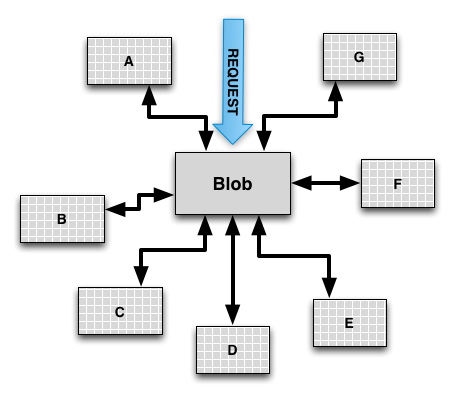
\includegraphics[width=1\textwidth]{./images/BLOB.png}
\caption{The God class\cite{Wert2013a}. }
\label{fig:godclass}
\end{minipage}
\begin{minipage}{.5\textwidth}
\centering
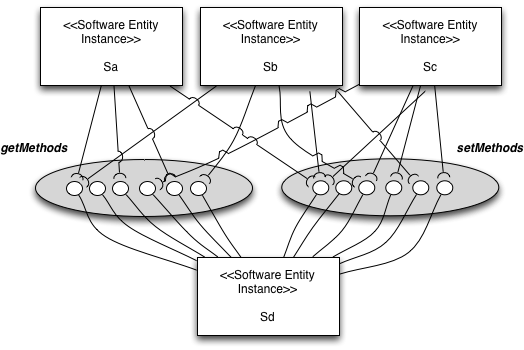
\includegraphics[width=1\textwidth]{./images/blob2.png}
\caption{The God class\cite{Vetoio2011}. }
\label{fig:godclass2}
\end{minipage}
\end{figure}

Unbalanced Processing it's characterises for one scenario where a specific class of requests generates a pattern of execution within the system that tends to overload a particular resource. In other words the overloaded resource will be executing a certain type of job very often, thus in practice damaging other classes
of jobs that will experience very long waiting times. Unbalanced Processing occurs in three different situations. The first case that cause unbalanced processing it is when processes cannot make effective use of available processors either because processors are dedicated to other tasks or because of single-threaded code. This manifestation has available processors and we need to ensure that the software is able to use them. Fig. \ref{fig:unbalanced}  shows a sample of the Unbalanced Processing. In The Fig. \ref{fig:unbalanced}, four tasks are performed. The task D it is waiting for the task C conclusion that are submmited to a heavy processing situation. 

The pipe and filter architectures  and extensive processing antipattern represents a manifestation of the unbalanced processing antipattern. The pipe and filter architectures occurs when the throughput of the overall system is determined by the slowest filter. The  Fig. \ref{fig:pipefilter} describes a software S with a Pipe and Filter Architectures problem: (a) Static View, there is a software entity instance, e.g. Sa, offering an operation (operation x) whose resource demand (computation = \$compOpx, storage = \$storOpx, bandwidth = \$bandOpx) is quite high; (b) Dynamic View, the operation opx is invoked in a service  and the throughput of the service (\$Th(S)) is lower than the required one. The extensive processing occurs when a process monopolizes a processor and prevents a set of other jobs to be executed until it finishes its computation. The Fig. \ref{fig:extpro} describes a software S with a Extensive Processing problem: (a) Static View, there is a software entity instance, e.g. Sa, offering two operations (operation x, operation y) whose resource demand is quite unbalanced, since opx has a high demand (computation = \$compOpx, storage = \$storOpx, bandwidth = \$bandOpx), whereas opy has a low demand (computation = \$compOpy, storage = \$storOpy, bandwidth = \$bandOpy); (b) Dynamic View, the operations opx and opy are alternatively invoked in a service and the response time of the service (\$RT(S)) is larger than the required one \cite{Vetoio2011}.

\begin{figure}[h]
\centering
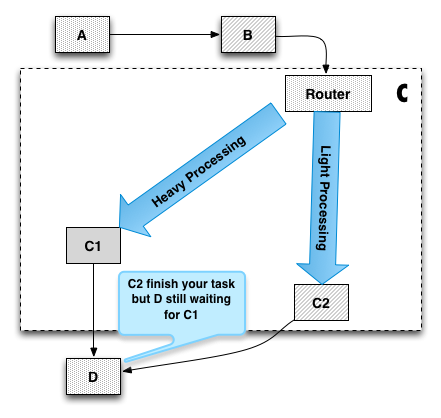
\includegraphics[width=0.5\textwidth]{./images/unbalanced.png}
\caption{Unbalanced Processing sample \cite{Wert2013a}. }
\label{fig:unbalanced}
\end{figure}


\begin{figure}[h]
\begin{minipage}{.5\textwidth}
\centering
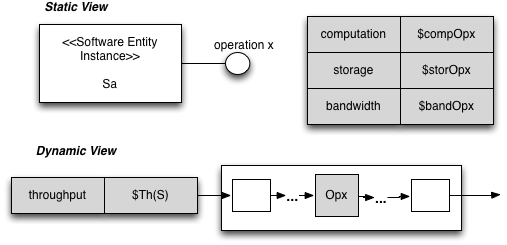
\includegraphics[width=1\textwidth]{./images/pipe2.png}
\caption{Pipe and Filter sample \cite{Vetoio2011}}
\label{fig:pipefilter}
\end{minipage}
\begin{minipage}{.5\textwidth}
\centering
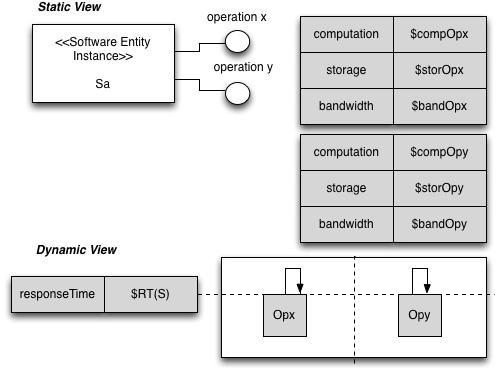
\includegraphics[width=1\textwidth]{./images/extpro.png}
\caption{Extensive Processing sample \cite{Vetoio2011}.}
\label{fig:extpro}
\end{minipage}
\end{figure}


Circuitous Treasure Hunt antipattern occurs when software retrieves data from a first componet, uses those results in a second component, retrieves data from the second component, and so on, until the last results are obtained \cite{Smith2002} \cite{Smith2003}. Circuitous Treasure Hunt 
are typical performance antipatterns that causes unnecessarily frequent database requests. The Circuitous Treasure Hunt antipattern is a result from a bad database schema or query design. A common Circuitous Treasure Hunt design creates a data dependency between single queries. For instance, a query requires the
result of a previous query as input. The longer the chain of
dependencies between individual queries the more the Circuitous
Treasure Hunt antipattern hurts performance \cite{Wert2014}. The Fig. \ref{fig:circuit}  shows a software S with a Circuitous Treasure Hunt problem: (a) Static View, there is a software entity instance e.g. Sa, retrieving information from the database; (b) Dynamic View, the software  S generates a large number of database calls by performing several queries up to the final operation \cite{Vetoio2011}.


\begin{figure}[h]
\begin{minipage}{.5\textwidth}
\centering
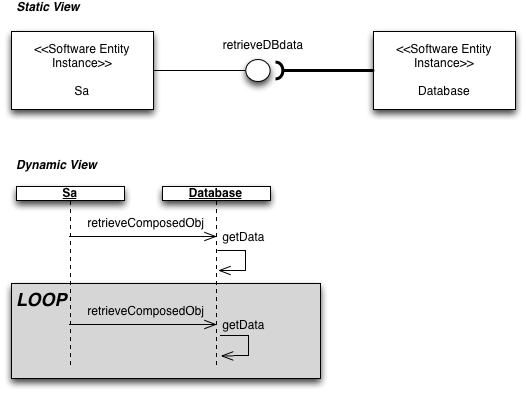
\includegraphics[width=1\textwidth]{./images/circuit.png}
\caption{Circuitous
Treasure Hunt sample \cite{Vetoio2011}}
\label{fig:circuit}
\end{minipage}
\begin{minipage}{.5\textwidth}
\centering
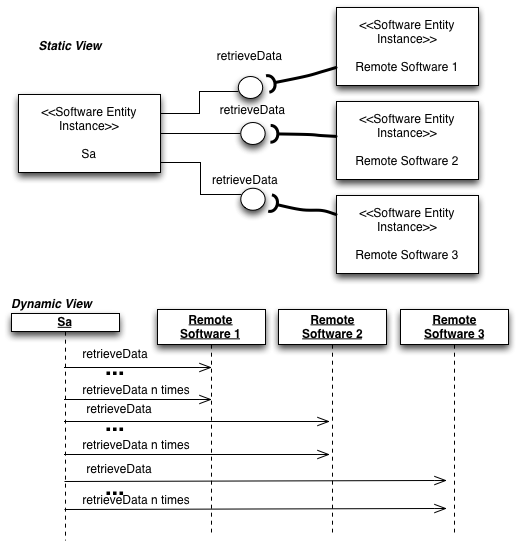
\includegraphics[width=1\textwidth]{./images/trucks.png}
\caption{Empty Semi Trucks sample \cite{Vetoio2011}.}
\label{fig:trucks}
\end{minipage}
\end{figure}

Empty Semi Trucks occurs when an excessive number of requests is required to perform a task. It may be due to inefficient use of available bandwidth, an inefficient interface, or both \cite{Arcelli2012}. There are a special case of Empty Semi Trucks that occurs  when many fields in a user interface must be retrieved from a
remote system. Fig. shows a software S with a Empty Semi Trucks problem: (a) Static View, there is a software entity instance, e.g. Sa, retrieving some information from several instances (Remote Software 1, . . . , Remote Software n); (b) Dynamic View, the software instance Sa generates an excessive message traffic by sending a big amount of messages with low sizes, much lower than the network bandwidth, hence the network link might have a low utilization value \cite{Vetoio2011}.

The Tower of Babel antipattern most often occurs when information is translated into an exchange format, such as XML, by the sending process then parsed and translated into an
internal format by the receiving process. When the translation and parsing is excessive, the system spends most
of its time doing this and relatively little doing real work \cite{Smith2003}. Fig. shows a system with a Tower of Babel problem: (a) Static View, there are some software entity instances, e.g. Sa, Sb, . . . , Sn; (b) Dynamic View, the software instances Sd performs many times the translation of format for communicating with other instances \cite{Vetoio2011}.

\begin{figure}[h]
\begin{minipage}{.5\textwidth}
\centering
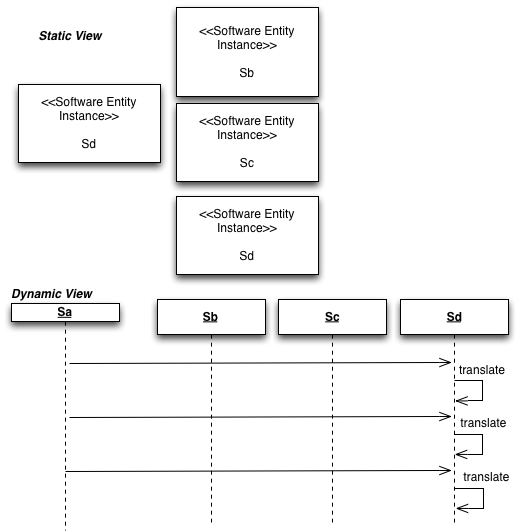
\includegraphics[width=1\textwidth]{./images/babel2.png}
\caption{Tower of Babel sample \cite{Vetoio2011}}
\label{fig:babel}
\end{minipage}
\begin{minipage}{.5\textwidth}
\centering
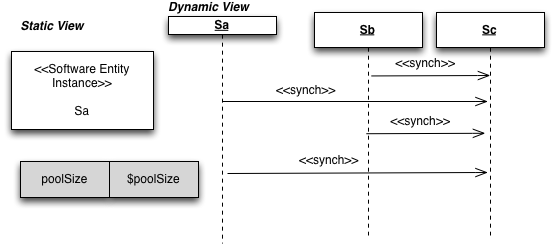
\includegraphics[width=1\textwidth]{./images/onelane.png}
\caption{One-Lane Bridge sample \cite{Vetoio2011}.}
\label{fig:onelane}
\end{minipage}
\end{figure}


One-Lane Bridge is a antipattern that occurs when one or a few processes execute concurrently using a shared resource and other processes are waiting for use the shared resource. It frequently occurs in applications that access a database. Here, a lock ensures that only one process may update the associated portion of the database at a time. This antipatterns is common when many concurrent threads or processes are waiting for the same shared resources. These can either be passive resources (like semaphores or mutexes) or active resources (like CPU or hard disk). In the first case, we have a typical One Lane Bridge whose critical resource needs to be identified. Figure 3.10 shows a system with a One-Lane Bridge problem: (a) Static View, there is a software entity instance with a capacity of managing \$poolSize threads; (b) Dynamic View, the software instance Sc receives an excessive number of synchronous calls in a service S and the predicted response time is higher than the required \cite{Vetoio2011}.


Using dynamic allocation, objects are created when they are first accessed and then destroyed when they are no longer needed. Excessive Dynamic Allocation, however, addresses frequent, unnecessary creation and destruction of objects of the same class. Dynamic allocation is expensive , an object created in memory must be allocated from the heap, and any initialization code for the object and the contained objects must be executed. When the object is no longer needed, necessary clean-up must be performed, and the reclaimed memory must be returned to the heap to avoid memory leaks \cite{Smith2002} \cite{Smith2003}.

\begin{figure}[H]
\begin{minipage}{.5\textwidth}
\centering
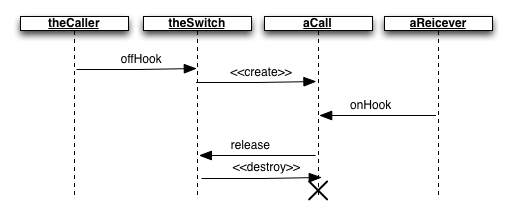
\includegraphics[width=1\textwidth]{./images/excessivedynamicallocation.png}
\caption{Excessive Dynamic Allocation.}
\label{fig:dynallocation}
\end{minipage}
\begin{minipage}{.5\textwidth}
\centering
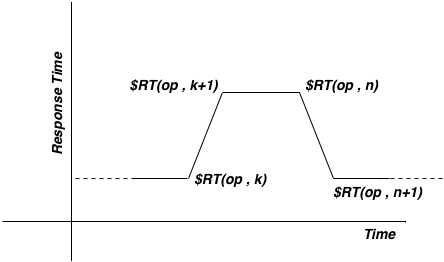
\includegraphics[width=1\textwidth]{./images/jam.png}
\caption{Traffic Jam Response Time \cite{Vetoio2011}.}
\label{fig:jam}
\end{minipage}
\end{figure}

The Fig. \ref{fig:dynallocation} shows a Excessive Dynamic Allocation sample. This example is drawn from a call (an offHook event), the switch creates a Call object to manage the call. When the call is completed, the Call object is destroyed. Constructing a single Call object it is not seem as excessive. A Call is a complex object that contains several other objects that must also be created. The Excessive Dynamic Allocation occurs when  a switch receive hundreds of thousands of offHook events. In a case like this, the overhead for dynamically allocating call objects adds substantial delays to the time needed to complete a call.

The Traffic Jam antipattern occurs if many concurrent threads or processes are waiting for the same  active resources (like CPU or hard disk). This antipatterns produces a large backlog in jobs waiting for service. The performance impact of the Traffic Jam is the transient behavior that produces wide variability in response time. Sometimes it is fine, but at other times, it is unacceptably long. Figure \ref{fig:jam} describes a software with a Traffic Jam problem, the monitored response time of the operation shows a wide variability in response time which persists long \cite{Vetoio2011}. 


\begin{figure}[H]
\begin{minipage}{.5\textwidth}
\centering
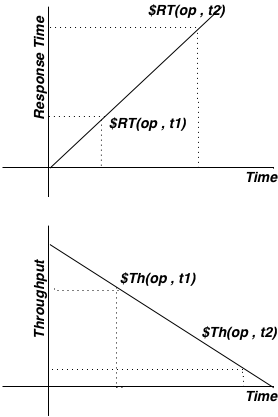
\includegraphics[width=0.5\textwidth]{./images/ramp.png}
\caption{The Ramp sample \cite{Vetoio2011}.}
\label{fig:ramp}
\end{minipage}
\begin{minipage}{.5\textwidth}
\centering
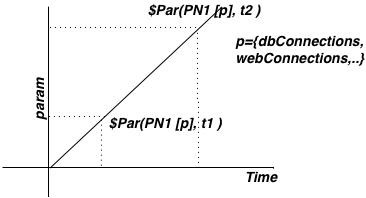
\includegraphics[width=1\textwidth]{./images/moreisless.png}
\caption{More is Less sample \cite{Vetoio2011}.}
\label{fig:moreisless}
\end{minipage}
\end{figure}

The Ramp it is a antipattern where the processing time increases as the system is used. The Ramp can arise in several different ways. Any situation in which the amount of processing required to satisfy a request increases over time will produce the behavior. With the Ramp antipattern, the memory consumption of the application is growing over time. The root cause is Specific Data Structures which are growing during operation or which are not properly disposed \cite{Wert2014} \cite{Smith2003}. Fig. \ref{fig:ramp} shows a system  with The Ramp problem:  (i) the monitored response time of the operation opx at time t1, i.e. \$RT(opx, t1), is much lower than the monitored response time of the operation opx at time t2, i.e. \$RT(opx, t2), with t1 < t2; (ii) the monitored throughput of the operation opx at time t1, i.e. \$Th(opx, t1), is much larger than the monitored throughput of the operation opx at time t2, i.e. \$Th(opx, t2), with t1 < t2. 

More is less occurs when a system spends more time "thrashing” than accomplishing real work because there are too many processes relative to available resources. More is Less are presented when it is running too many programs overtime. This antipattern causes too much system paging and systems spend all their time servicing page faults rather than processing requests. In distributed systems, there are more causes.They include: creating too many database connections and  allowing too many internet connection. Fig. \ref{fig:moreisless} describes a system  with a More Is Less problem: There is a processing node PN1 and the monitored runtime parameters (e.g. database connections, etc.) at time t1, i.e. \$Par(PN1[p], t1), are much larger than the same parameters at time t2, i.e. \$Par(PN1[p], t2), with t1 < t2. 


To emulate the presented antipatterns the testbed solution uses Mock Objects with the JMeter load test tool.


